\chapter{Visualizing viral spread in time and space\label{chap:spread}}

\begin{remark}{Outline}
This chapter is adapted from the following publication: \\
F. Bielejec, A. Rambaut, M.A. Suchard and P. Lemey.
SPREAD: spatial phylogenetic reconstruction of evolutionary dynamics.
Bioinformatics, 2011, 27(20): 2910 -- 2912
\end{remark}

\section{Abstract}

\textbf{Summary:}\\
SPREAD is a user-friendly, cross-platform application to analyze and visualize Bayesian phylogeographic reconstructions incorporating spatial-temporal diffusion.
The software maps phylogenies annotated with both discrete and continuous spatial information and can export high-dimensional posterior summaries to keyhole markup language (KML) for animation of the spatial diffusion through time in virtual globe software.
In addition, SPREAD implements Bayes factor calculation to evaluate the support for hypotheses of historical diffusion among pairs of discrete locations based on Bayesian stochastic search variable selection estimates.
SPREAD takes advantage of multi-core architectures to process large joint posterior distributions of phylogenies and their spatial diffusion and produces visualizations as compelling and interpretable statistical summaries for the different spatial projections.\\

\noindent
\textbf{Availability:} \\
SPREAD is licensed under the GNU Lesser GPL and its source code is freely available as a GitHub repository: \url{https://github.com/phylogeography/SPREAD} 
Compiled, runnable package and supplementary data are hosted at: \url{http://rega.kuleuven.be/cev/ecv/software/spread} 

\begin{figure}[h!]
\centering
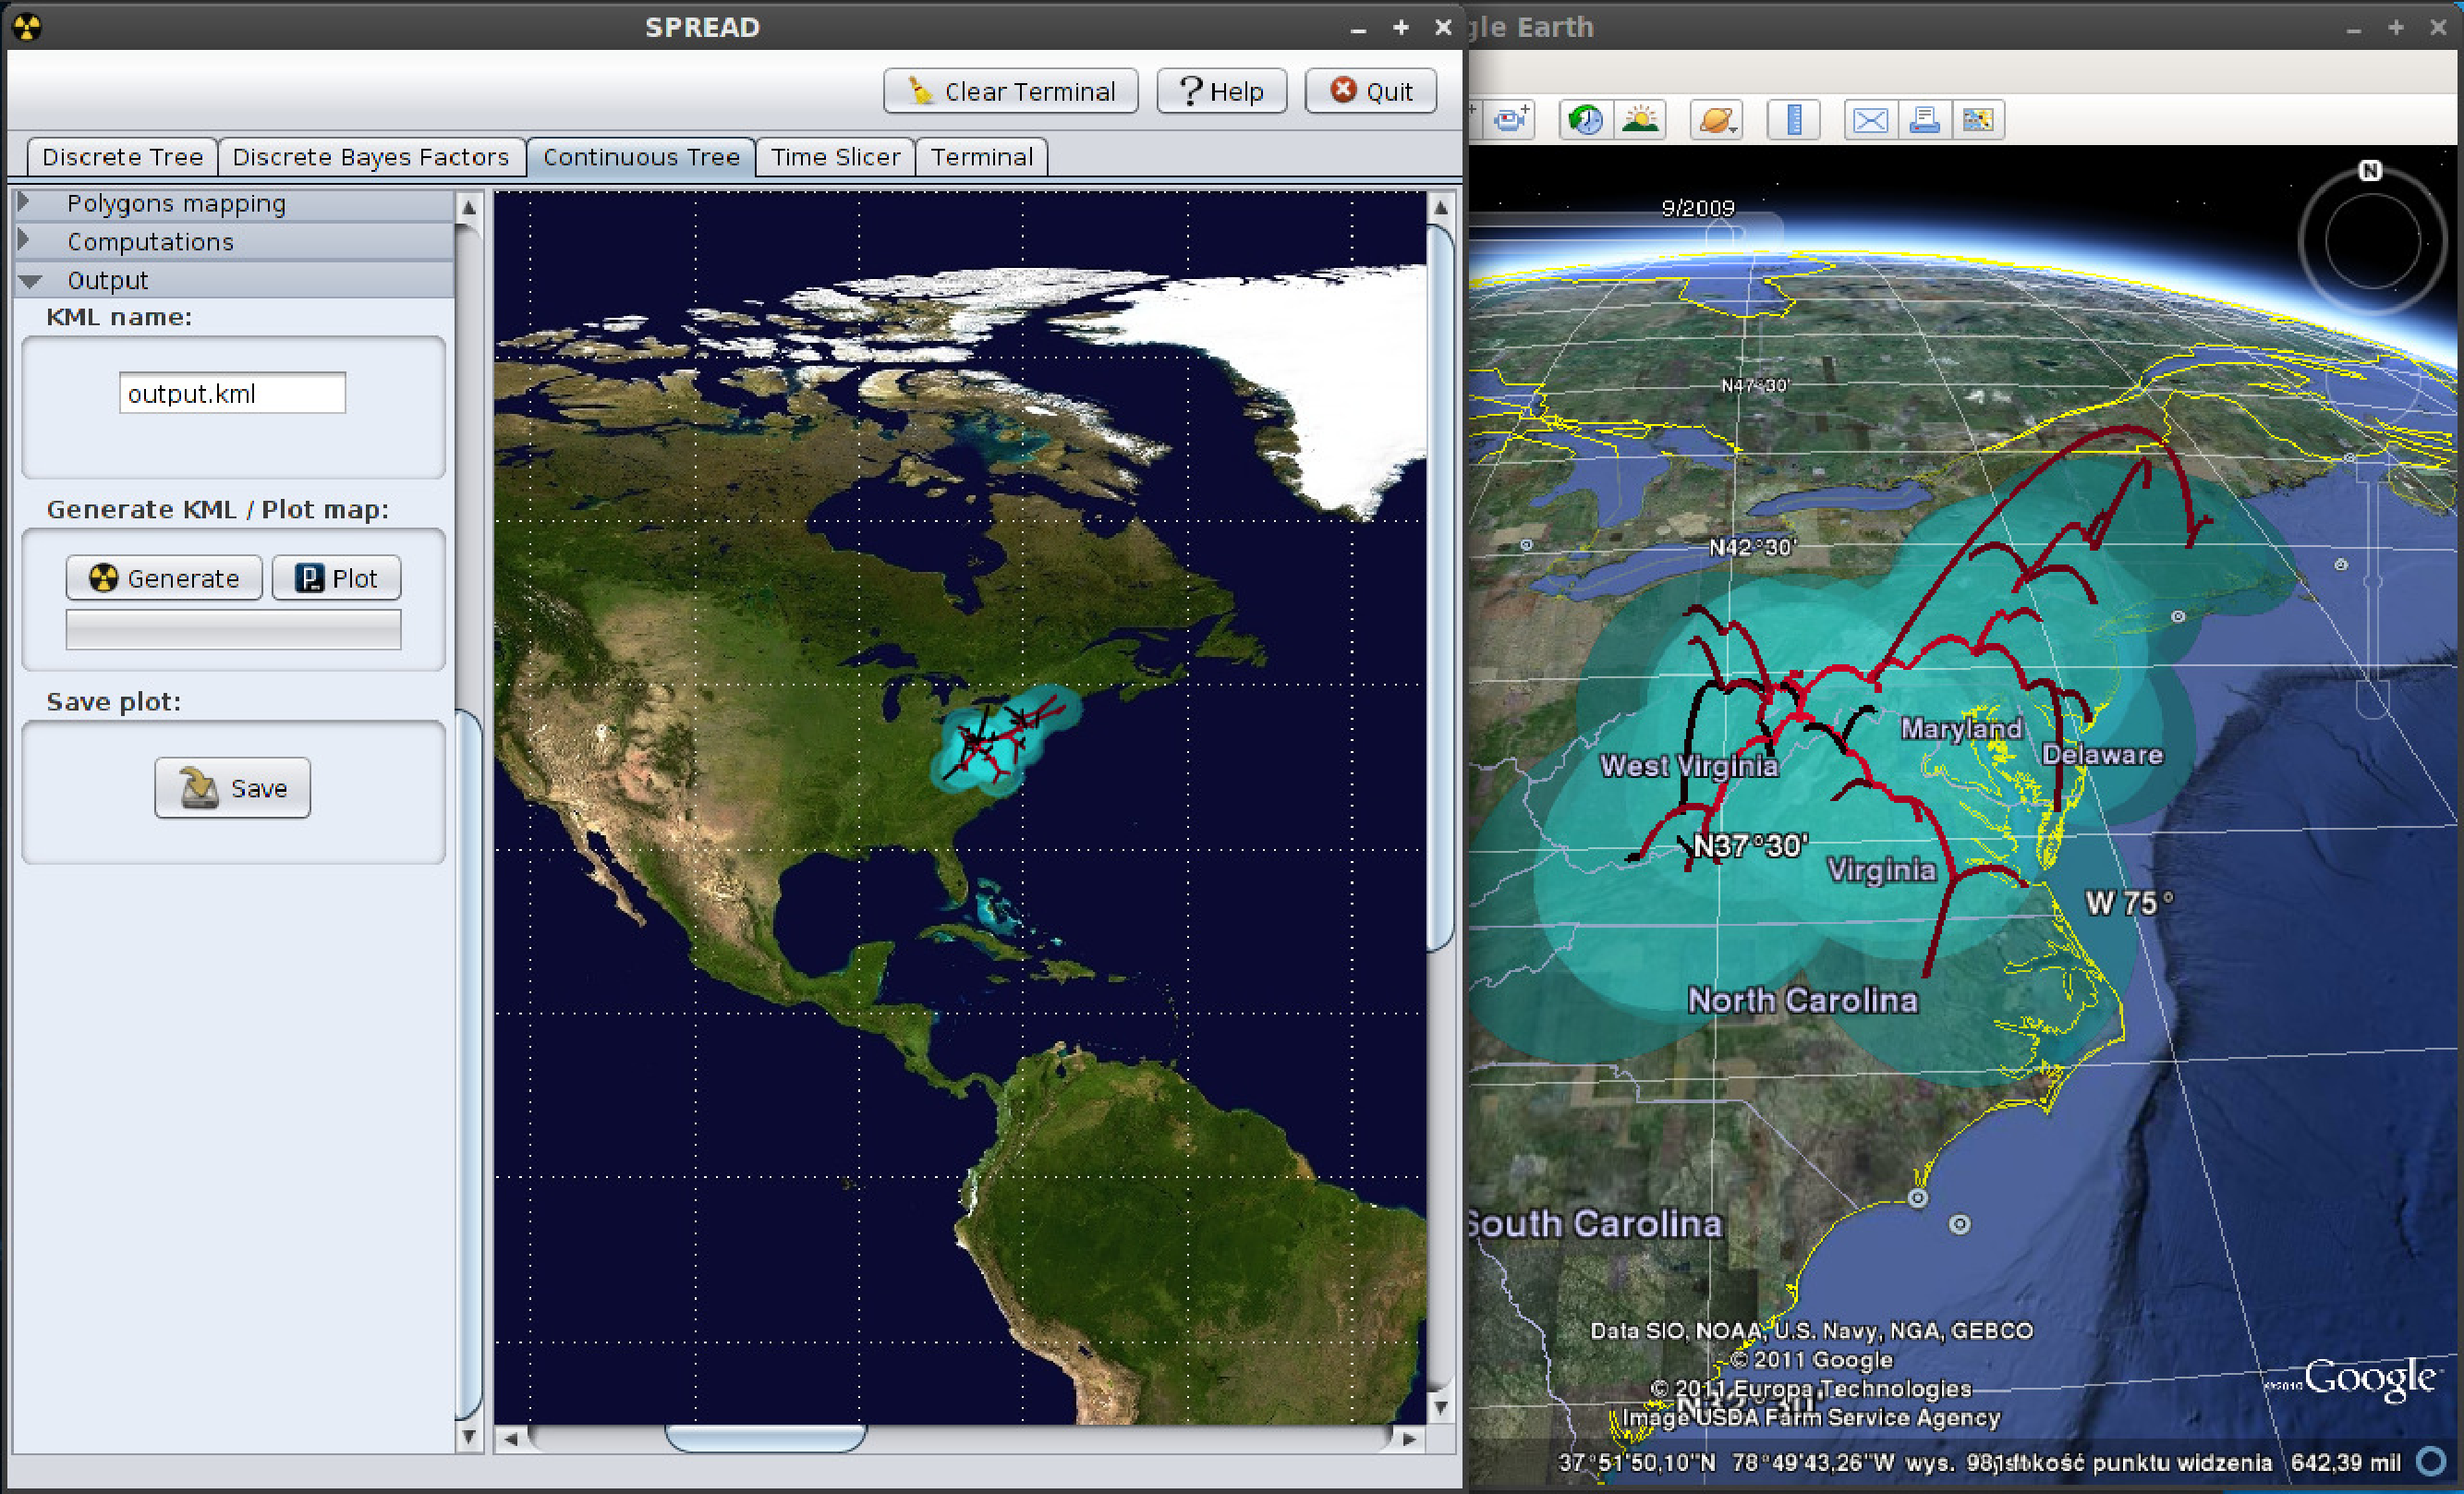
\includegraphics[scale=0.25]{RacRABV_cont_vis-color}
\caption{
{ \footnotesize 
{\bf Screenshot of SPREAD.}
This example visualizes the phylogeographic history of rabies among raccoons along the Eastern US seaboard under a continuous diffusion model.  Such visualizations allow users to quickly inspect key evolutionary changes in their geographic context.  Further generation of KML output enables interactive exploration in the time-dimension as well in freely available virtual globe software, such as {\sc Google Earth} (on right).
}% END: footnotesize 
}
\label{fig:screenshot01}
\end{figure}

\section{Introduction}

The advent of powerful and flexible Geographic Information Systems (GIS) has fostered an increasing interest in incorporating geographical information into molecular phylogenetic methods.
Spatial phylogenetic projections in a cartographic background play an important role in these developments \citep{Kidd2006, Parks2009}, but most applications remain limited to mapping phylogenetic tip taxa to their geographical coordinates.
Mapping phylogeographic histories of geo-referenced taxa requires a robust statistical estimate of the geographic locations at the ancestral nodes of the tree. 
To obtain such estimates under stochastic process-driven models, we recently proposed a suite of Bayesian inference approaches for the joint reconstruction of evolutionary and geographic history \citep{Lemey2009,Lemey2010, Bloomquist2010}.
Models that accommodate spatial diffusion in discrete and continuous space have been implemented in a flexible Bayesian statistical framework (BEAST, \cite{Drummond2007}, \url{http://beast.bio.ed.ac.uk}) for hypothesis testing based on time-measured evolutionary histories.
These approaches produce statistical distributions of temporal-spatial phylogenies and this has created new challenges for statistical phylogenetics in producing informative and compelling visualizations.
Here, we present software to fully exploit spatio-temporal annotations on phylogenies by providing flexible visual summaries that can be further examined in an interactive manner using GIS or virtual globe software.
A tutorial that explains how to use the software is included as Appendix~\ref{app:spread_tuto}.

\section{Features}

SPREAD provides four templates to analyze and visualize different aspects of phylogeographic diffusion, labeled: \textbf{Discrete Tree}, \textbf{Discrete Bayes Factors}, \textbf{Continuous Tree} and \textbf{Time Slicer}.
The discrete and continuous tree templates typically provide posterior summaries of diffusion from a Bayesian analysis along a \newline 
high-probability tree, such as the maximum clade credibility (MCC) tree of BEAST. 
However, SPREAD is not necessarily limited to this input, as it employs a general, trait-annotated NEXUS format; we provide several tree file examples in the supplementary information for both discrete or continuous annotations. 
SPREAD supports customized visualization of spatially-mapped trees, including branch coloring according to time and branch width manipulation.

\textbf{Discrete Tree} associates geographic coordinates with the discrete location states annotated to tree nodes and projects branches that accommodate location changes on a map.
Branches that maintain a location state are visualized using customizable circular polygons.

\textbf{Discrete Bayes Factors} summarizes the data support for each pairwise rate of diffusion between locations based on Bayesian stochastic search variable selection estimates inferred using BEAST.
This template takes as input a posterior sample of rate indicators from an augmented continuous-time Markov chain model and the Poisson prior specifications for the total number of non-zero rates.
\cite{Lemey2009} describe the Bayes factor calculations in more detail.

\textbf{Continuous Tree} maps all branches of a continuous diffusion phylogeography and allows plotting the uncertainty of geographic coordinates at the internal nodes through their annotated highest posterior density contours.

\textbf{Time Slicer} supplements the visualization of geographic locations estimated using continuous diffusion by summarizing the rate and degree of geographical movement over the complete posterior distribution of trees.
To obtain such ranges, we slice each rooted tree in the posterior sample at a number of points within a time interval, usually defined by the length of a summary (MCC) tree, and impute the unobserved ancestral locations for each branch that intersects those time points. To fully accommodate the uncertainty of the original inference, the imputation involves building Brownian bridges that can take into account branch-specific scaling factors of diffusion rates under relaxed random walks \citep{Lemey2010}. For each time point, we collect the imputed locations across the posterior distribution and use bivariate kernel density estimates to plot the highest posterior density contours.
The kernel density estimation follows \cite{Snyder1978} and uses bivariate normal kernels with a diagonal bandwidth with bandwidths based on Silverman's ``rule-of-thumb''  plug-in value \citep{Silverman1986}.

\section{Example and perspectives}

For all four template analyses, SPREAD offers direct visualization but also can export the mapped objects to a keyhole markup language (KML) file suitable for viewing with virtual globe software, such as Google Earth (\url{http://earth.google.com}).
A limited example on raccoon rabies diffusion \citep{Lemey2009} finds itself in Figure~\ref{fig:screenshot01};
dynamic visualizations of this example as well as others are provided at \url{http://rega.kuleuven.be/cev/ecv/software/spread}.
KML files can be imported and visualized by many GIS software packages, including ARCGIS and Cartographica.  

SPREAD is generally not the run-time limiting analysis, compared to fitting the original phylogenetic model, and readily accommodates larger problems.
Even for Bayesian phylogenetic analyses, 1000s of pathogen sequences can be accommodated, e.g. \cite{Rambaut2008}, and new computational technologies are actively stretching these limits \citep{Suchard2009}.
Future developments of SPREAD are aimed at extending built-in rendering functionality such as parsing custom base-maps and adding mouse-driven camera support to the embedded renderings. 
